\documentclass[10pt,a4paper]{article}
\usepackage[margin=17mm,top=15mm,bottom=16mm]{geometry}
\usepackage[T1]{fontenc}
\usepackage{newpxtext,newpxmath}
\usepackage{microtype}
\usepackage{amsmath,mathtools}
\usepackage{xcolor}
\usepackage{tikz}
\usepackage[most]{tcolorbox}
\usepackage{enumitem,multicol,fancyhdr,booktabs,array}
\usepackage[hidelinks]{hyperref}
\usetikzlibrary{arrows.meta,calc,positioning,patterns,decorations.pathreplacing}

\definecolor{navy}{HTML}{102A43}
\definecolor{ink}{HTML}{18323F}
\definecolor{muted}{HTML}{607684}
\definecolor{line}{HTML}{D8E2E8}
\definecolor{blue}{HTML}{2D72D9}
\definecolor{teal}{HTML}{008F83}
\definecolor{gold}{HTML}{E5A43A}
\definecolor{coral}{HTML}{E66555}
\definecolor{pale}{HTML}{F4F8FA}
\definecolor{paleblue}{HTML}{EAF3FF}
\definecolor{paleteal}{HTML}{E6F7F4}
\definecolor{palegold}{HTML}{FFF4DC}
\definecolor{palecoral}{HTML}{FCEBE8}

\color{ink}\setlength{\parindent}{0pt}\setlength{\parskip}{3pt}\linespread{1.025}
\setlist[itemize]{leftmargin=14pt,itemsep=2pt,topsep=3pt}
\setlist[enumerate]{leftmargin=18pt,itemsep=2pt,topsep=3pt}
\DeclareMathOperator{\meas}{m}
\newcommand{\R}{\mathbb R}
\newcommand{\B}{\mathcal B}
\newcommand{\1}{\mathbf 1}
\newcommand{\dd}{\,\mathrm d}

\pagestyle{fancy}\fancyhf{}\renewcommand{\headrulewidth}{0pt}\renewcommand{\footrulewidth}{.45pt}
\fancyfoot[L]{\fontsize{7}{8}\selectfont\color{muted}\footertext}
\fancyfoot[R]{\fontsize{7}{8}\selectfont\color{muted}\thepage\,/\,13}
\newcommand{\footertext}{LEBESGUE INTEGRATION}
\newcommand{\pagehead}[3]{{\fontsize{7.2}{8}\selectfont\bfseries\color{teal}#1\quad #2\hfill\normalfont\color{muted}A VISUAL GUIDE TO LEBESGUE INTEGRATION}\par\vspace{2pt}{\color{line}\hrule height .45pt}\vspace{8pt}{\fontsize{22}{24}\selectfont\bfseries\color{navy}#3}\par\vspace{5pt}}
\newcommand{\lead}[1]{{\fontsize{11.2}{15}\selectfont #1\par}\vspace{5pt}}
\newcommand{\eyebrow}[1]{{\fontsize{7}{8}\selectfont\bfseries\color{teal}\MakeUppercase{#1}}}
\newtcolorbox{mathbox}[1][]{enhanced,boxrule=0pt,arc=6pt,colback=paleblue,left=9pt,right=9pt,top=7pt,bottom=7pt,#1}
\newtcolorbox{tealbox}[1][]{enhanced,boxrule=0pt,arc=6pt,colback=paleteal,left=9pt,right=9pt,top=7pt,bottom=7pt,#1}
\newtcolorbox{goldbox}[1][]{enhanced,boxrule=0pt,arc=6pt,colback=palegold,left=9pt,right=9pt,top=7pt,bottom=7pt,#1}
\newtcolorbox{coralbox}[1][]{enhanced,boxrule=0pt,arc=6pt,colback=palecoral,left=9pt,right=9pt,top=7pt,bottom=7pt,#1}
\newtcolorbox{quietbox}[1][]{enhanced,boxrule=.45pt,arc=6pt,colback=pale,colframe=line,left=8pt,right=8pt,top=7pt,bottom=7pt,#1}
\tikzset{flow/.style={-{Stealth[length=5pt]},draw=teal,line width=1.1pt},axis/.style={draw=line,line width=.5pt},bluecurve/.style={draw=blue,line width=1.5pt},tealcurve/.style={draw=teal,line width=1.5pt}}
\hypersetup{pdftitle={Lebesgue Integration: Measure, Approximation, and Convergence},pdfauthor={Benjamin Michael Haire},pdfsubject={A visual guide to Lebesgue integration with worked examples},pdfkeywords={Lebesgue integral, measure theory, measurable functions, convergence theorems}}

\begin{document}
\thispagestyle{empty}\pagecolor{navy}\color{white}
\vspace*{8mm}
{\fontsize{7.5}{9}\selectfont\bfseries\color{teal!55!white}VISUAL MATHEMATICS\quad/\quad THEORY + CALCULATION\quad/\quad LATEX EDITION}\par
\vspace{10mm}
{\fontsize{35}{36}\selectfont\bfseries Lebesgue\par integration}\par
\vspace{5mm}
{\fontsize{13}{18}\selectfont\color{white!82}Measure the domain by the values a function takes. Build the integral from measurable sets, then pass safely to limits.}\par
\vspace{15mm}
\begin{center}
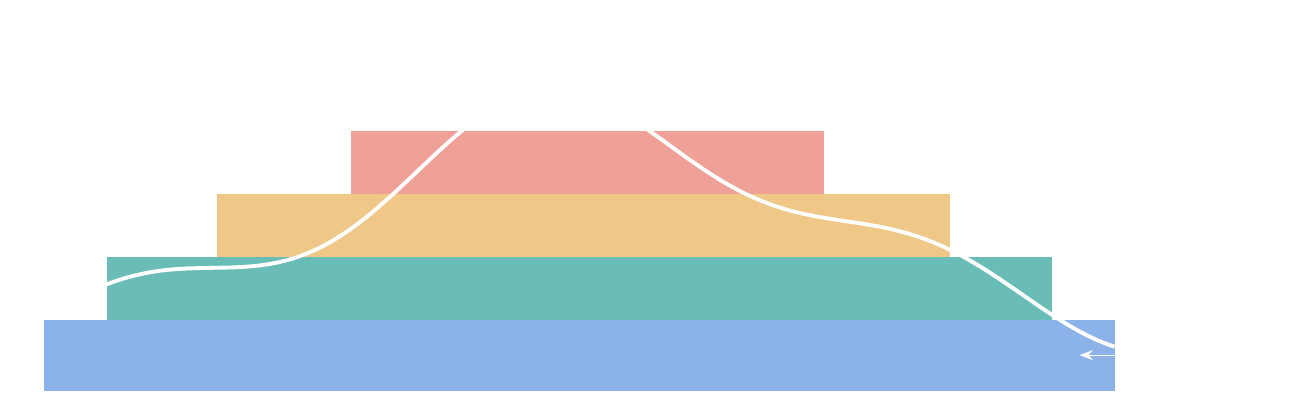
\begin{tikzpicture}[x=1cm,y=1cm]
  \draw[draw=white!25,line width=.5pt] (0,0) rectangle (14,4.6);
  \foreach \x in {0.2,0.35,...,13.8} {\pgfmathsetmacro\h{.7+2.8*exp(-0.06*(\x-7)^2)+.35*sin(70*\x)}\draw[white!40,line width=.32pt] (\x,0)--(\x,\h);}
  \fill[blue!70,opacity=.78] (.2,0) rectangle (13.8,.9);
  \fill[teal!75,opacity=.78] (1.0,.9) rectangle (13.0,1.7);
  \fill[gold!75,opacity=.82] (2.4,1.7) rectangle (11.7,2.5);
  \fill[coral!75,opacity=.82] (4.1,2.5) rectangle (10.1,3.3);
  \draw[white,line width=1.4pt,domain=.2:13.8,samples=120] plot (\x,{.7+2.8*exp(-0.06*(\x-7)^2)+.35*sin(70*\x)});
  \node[anchor=west,text=white!80,font=\scriptsize] at (14.15,.45) {value bands};
  \draw[-{Stealth},white!65] (14.05,.45)--(13.35,.45);
\end{tikzpicture}
\end{center}
\vfill
{\fontsize{14}{17}\selectfont\bfseries The governing idea}\par\vspace{2mm}
{\fontsize{10.5}{14}\selectfont\color{white!82}Riemann cuts the \emph{horizontal axis} into intervals. Lebesgue groups points of the domain by \emph{height}. The integral becomes a weighted sum: height $\times$ the measure of the set carrying that height.}\par
\vspace{9mm}{\fontsize{7}{8}\selectfont\color{white!58}Prerequisites: limits, series, and basic real analysis\hfill Benjamin Michael Haire / 2026}
\newpage\nopagecolor\color{ink}

\renewcommand{\footertext}{WHY A NEW INTEGRAL? / HORIZONTAL VERSUS VERTICAL SLICING}
\pagehead{01}{THE CHANGE OF VIEWPOINT}{Partition the range, not the domain}
\lead{Both theories seek area. Their bookkeeping differs: Riemann samples thin vertical strips; Lebesgue measures the sets on which the function has comparable values.}
\begin{center}
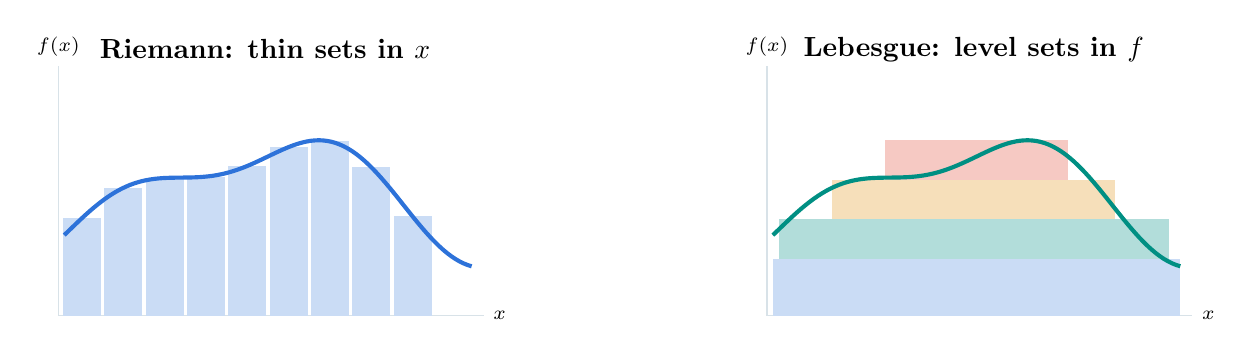
\begin{tikzpicture}[x=.75cm,y=.72cm]
\begin{scope}
 \draw[axis] (0,0)--(7.2,0) node[right,font=\scriptsize] {$x$}; \draw[axis] (0,0)--(0,4.4) node[above,font=\scriptsize] {$f(x)$};
 \foreach \x in {.4,1.1,...,6.7}{\pgfmathsetmacro\h{1.1+2.0*exp(-.18*(\x-3.5)^2)+.45*sin(90*\x)}\fill[blue!25] (\x-.32,0) rectangle (\x+.32,\h);}
 \draw[bluecurve,domain=.1:7,samples=100] plot (\x,{1.1+2.0*exp(-.18*(\x-3.5)^2)+.45*sin(90*\x)});
 \node[font=\bfseries] at (3.5,4.7) {Riemann: thin sets in $x$};
\end{scope}
\begin{scope}[xshift=9cm]
 \draw[axis] (0,0)--(7.2,0) node[right,font=\scriptsize] {$x$}; \draw[axis] (0,0)--(0,4.4) node[above,font=\scriptsize] {$f(x)$};
 \fill[blue!25] (.1,0) rectangle (7,1.0); \fill[teal!30] (.2,1) rectangle (6.8,1.7); \fill[gold!35] (1.1,1.7) rectangle (5.9,2.4); \fill[coral!35] (2.0,2.4) rectangle (5.1,3.1);
 \draw[tealcurve,domain=.1:7,samples=100] plot (\x,{1.1+2.0*exp(-.18*(\x-3.5)^2)+.45*sin(90*\x)});
 \node[font=\bfseries] at (3.5,4.7) {Lebesgue: level sets in $f$};
\end{scope}
\end{tikzpicture}
\end{center}
\begin{minipage}[t]{.48\textwidth}\begin{quietbox}\textbf{What Riemann needs}\par Bounded functions with discontinuities confined to a set of measure zero are Riemann integrable. Dense or wild discontinuities can defeat its interval sums.\end{quietbox}\end{minipage}\hfill
\begin{minipage}[t]{.48\textwidth}\begin{tealbox}\textbf{What Lebesgue gains}\par It integrates many limits of functions, treats null sets as negligible, and turns convergence into a systematic theory. Every Riemann-integrable function is Lebesgue integrable with the same value.\end{tealbox}\end{minipage}
\vspace{5pt}
\begin{mathbox}\centering
\textbf{Layer-cake intuition:}\qquad $\displaystyle \int_X f\dd\mu=\int_0^\infty \mu\{x:f(x)>t\}\dd t\quad(f\ge0)$.
\end{mathbox}
\newpage

\renewcommand{\footertext}{SIGMA-ALGEBRAS / MEASURES / NULL SETS}
\pagehead{02}{THE MEASURABLE WORLD}{Which sets may receive a size?}
\lead{A measure is not assigned to every imaginable subset. We first select a stable collection of measurable sets, then require size to add over disjoint countable unions.}
\begin{center}
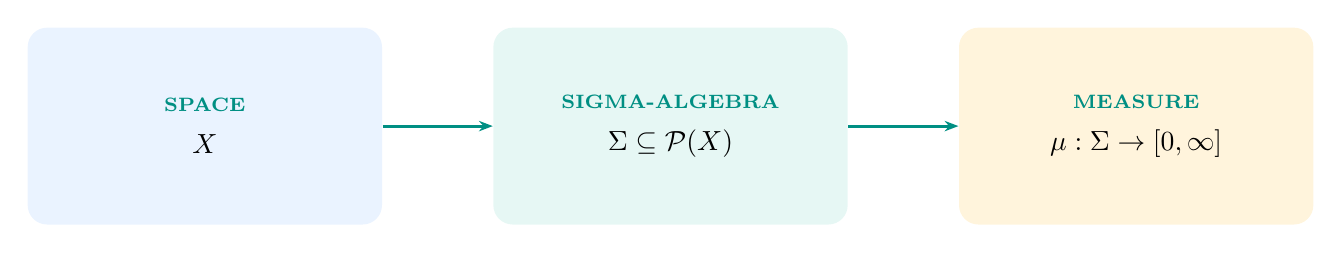
\begin{tikzpicture}[node distance=14mm]
\node[rounded corners=7pt,fill=paleblue,minimum width=45mm,minimum height=25mm,align=center] (x) {\eyebrow{Space}\\[3pt]$X$};
\node[rounded corners=7pt,fill=paleteal,minimum width=45mm,minimum height=25mm,align=center,right=of x] (s) {\eyebrow{Sigma-algebra}\\[3pt]$\Sigma\subseteq\mathcal P(X)$};
\node[rounded corners=7pt,fill=palegold,minimum width=45mm,minimum height=25mm,align=center,right=of s] (m) {\eyebrow{Measure}\\[3pt]$\mu:\Sigma\to[0,\infty]$};
\draw[flow] (x)--(s);\draw[flow] (s)--(m);
\end{tikzpicture}
\end{center}
\begin{minipage}[t]{.48\textwidth}
\begin{mathbox}\textbf{$\sigma$-algebra axioms}\par
$X\in\Sigma$; if $A\in\Sigma$, then $A^c\in\Sigma$; and if $A_n\in\Sigma$, then $\bigcup_{n=1}^{\infty}A_n\in\Sigma$. Consequently it is also closed under countable intersections and differences.\end{mathbox}
\end{minipage}\hfill
\begin{minipage}[t]{.48\textwidth}
\begin{tealbox}\textbf{Measure axioms}\par
$\mu(\varnothing)=0$ and, for pairwise disjoint $A_n$,
\[\mu\!\left(\bigcup_{n=1}^\infty A_n\right)=\sum_{n=1}^\infty\mu(A_n).\]
Monotonicity and countable subadditivity follow.\end{tealbox}
\end{minipage}
\vspace{6pt}
\begin{goldbox}\eyebrow{On the real line}\par
The Borel sets $\B(\R)$ are generated by open intervals. Lebesgue measure $m$ extends interval length, $m([a,b])=b-a$, to the completed Borel $\sigma$-algebra, including all subsets of null sets. Countable sets have measure zero, yet $\R\setminus\mathbb Q$ has full measure in every interval.\end{goldbox}
\begin{coralbox}\textbf{Almost everywhere (a.e.).} A statement holds almost everywhere when its exceptional set has measure zero. Lebesgue integration identifies functions that differ only on a null set: changing finitely or countably many values does not change the integral.\end{coralbox}
\newpage

\renewcommand{\footertext}{MEASURABLE FUNCTIONS / PREIMAGES / SIMPLE FUNCTIONS}
\pagehead{03}{FUNCTIONS THAT RESPECT MEASURE}{Measurability is a preimage condition}
\lead{A function is measurable when asking whether its value falls below a threshold always produces a measurable subset of the domain.}
\begin{mathbox}\centering
$f:(X,\Sigma)\to(\R,\B(\R))$ is measurable $\Longleftrightarrow$ $\{x:f(x)>a\}\in\Sigma$ for every $a\in\R$.
\end{mathbox}
\begin{center}
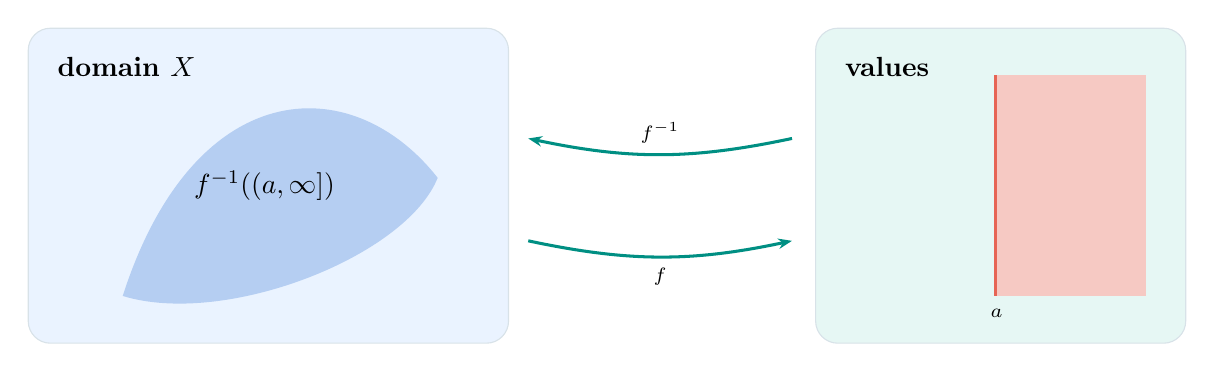
\begin{tikzpicture}[x=1cm,y=1cm]
 \draw[rounded corners=8pt,fill=paleblue,draw=line] (0,0) rectangle (6.1,4);
 \draw[rounded corners=8pt,fill=paleteal,draw=line] (10,0) rectangle (14.7,4);
 \fill[blue!35] (1.2,.6) .. controls (2.5,.2) and (4.8,1.1) .. (5.2,2.1) .. controls (4.1,3.5) and (2.1,3.4) .. (1.2,.6);
 \node at (3,2) {$f^{-1}((a,\infty])$}; \node[anchor=north west,font=\bfseries] at (.25,3.75) {domain $X$};
 \draw[coral,line width=2pt] (12.3,.6)--(12.3,3.4); \fill[coral!35] (12.3,.6) rectangle (14.2,3.4);
 \node[font=\scriptsize,below] at (12.3,.55) {$a$}; \node[anchor=north west,font=\bfseries] at (10.25,3.75) {values};
 \draw[flow] (9.7,2.6) to[bend left=12] node[above,font=\scriptsize] {$f^{-1}$} (6.35,2.6);
 \draw[flow] (6.35,1.3) to[bend right=12] node[below,font=\scriptsize] {$f$} (9.7,1.3);
\end{tikzpicture}
\end{center}
\begin{tealbox}\eyebrow{The first integrable building blocks}\par
A nonnegative simple function has finitely many heights:
\[s(x)=\sum_{k=1}^n a_k\1_{A_k}(x),\qquad a_k\ge0,\ A_k\in\Sigma.\]
If the $A_k$ are disjoint, define $\displaystyle\int_Xs\dd\mu=\sum_{k=1}^n a_k\mu(A_k)$. Different representations give the same value.\end{tealbox}
\begin{quietbox}\textbf{Closure facts worth using.} Continuous functions are Borel measurable. Sums, products, pointwise suprema, pointwise limits, and positive/negative parts of measurable functions are measurable whenever defined.\end{quietbox}
\newpage

\renewcommand{\footertext}{THE DEFINITION / APPROXIMATION FROM BELOW}
\pagehead{04}{BUILDING THE INTEGRAL}{Simple functions climb from below}
\lead{For $f\ge0$, the integral is the largest area achieved by any measurable step function that never rises above $f$. This makes approximation part of the definition.}
\begin{mathbox}\centering
$\displaystyle \int_X f\dd\mu=\sup\left\{\int_Xs\dd\mu:0\le s\le f,\ s\text{ simple}\right\}\in[0,\infty].$
\end{mathbox}
\begin{center}
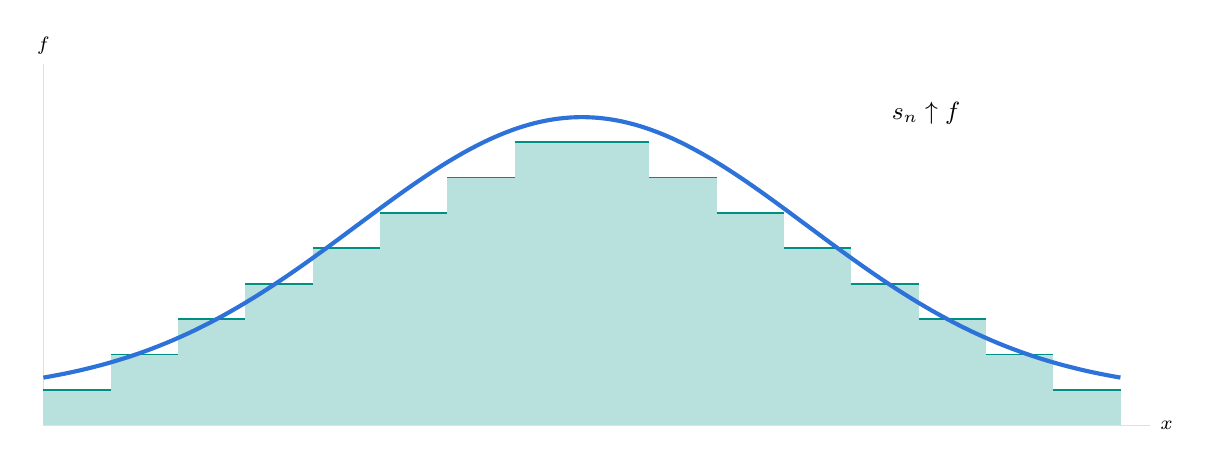
\begin{tikzpicture}[x=.95cm,y=.9cm]
 \draw[axis] (0,0)--(14.8,0) node[right,font=\scriptsize] {$x$}; \draw[axis] (0,0)--(0,5.1) node[above,font=\scriptsize] {$f$};
 \foreach \x/\w/\h in {0/.9/.5,.9/.9/1,1.8/.9/1.5,2.7/.9/2,3.6/.9/2.5,4.5/.9/3,5.4/.9/3.5,6.3/.9/4,7.2/.9/4,8.1/.9/3.5,9/.9/3,9.9/.9/2.5,10.8/.9/2,11.7/.9/1.5,12.6/.9/1,13.5/.9/.5}{\fill[teal!28] (\x,0) rectangle +(\w,\h);\draw[teal,line width=.65pt] (\x,\h)--+(\w,0);}
 \draw[bluecurve,domain=0:14.4,samples=150] plot (\x,{.45+3.9*exp(-.055*(\x-7.2)^2)});
 \node[fill=white,inner sep=2pt,font=\small] at (11.8,4.4) {$s_n\uparrow f$};
\end{tikzpicture}
\end{center}
\begin{minipage}[t]{.48\textwidth}\begin{goldbox}\textbf{Canonical approximation}\par For $f\ge0$, quantize heights in steps of $2^{-n}$ and truncate at $n$:
\[s_n=\begin{cases}2^{-n}\lfloor2^nf\rfloor,&f<n,\\ n,&f\ge n.\end{cases}\]
Then $0\le s_n\uparrow f$ pointwise.\end{goldbox}\end{minipage}\hfill
\begin{minipage}[t]{.48\textwidth}\begin{tealbox}\textbf{Signed functions}\par Split $f=f^+-f^-$, where $f^+=\max(f,0)$ and $f^-=\max(-f,0)$. Define
\[\int f=\int f^+-\int f^-\]
when at least one term is finite. The function is integrable when $\int|f|<\infty$.\end{tealbox}\end{minipage}
\newpage

\renewcommand{\footertext}{A PRACTICAL CALCULATION WORKFLOW}
\pagehead{05}{HOW TO CALCULATE}{Choose the shortest legitimate route}
\lead{In ordinary calculus problems, Lebesgue integrals often evaluate by familiar antiderivatives. The new theory matters most in deciding existence, ignoring null sets, interchanging limits, and handling irregular functions.}
\begin{center}
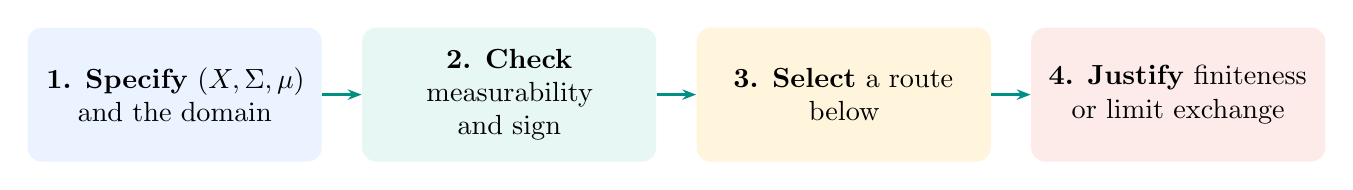
\begin{tikzpicture}[node distance=5mm]
\node[rounded corners=5pt,fill=paleblue,text width=35mm,minimum height=17mm,align=center] (a) {\textbf{1. Specify}\space $(X,\Sigma,\mu)$\\and the domain};
\node[rounded corners=5pt,fill=paleteal,text width=35mm,minimum height=17mm,align=center,right=of a] (b) {\textbf{2. Check}\space measurability\\and sign};
\node[rounded corners=5pt,fill=palegold,text width=35mm,minimum height=17mm,align=center,right=of b] (c) {\textbf{3. Select}\space a route\\below};
\node[rounded corners=5pt,fill=palecoral,text width=35mm,minimum height=17mm,align=center,right=of c] (d) {\textbf{4. Justify}\space finiteness\\or limit exchange};
\draw[flow] (a)--(b);\draw[flow] (b)--(c);\draw[flow] (c)--(d);
\end{tikzpicture}
\end{center}
\begin{minipage}[t]{.48\textwidth}
\begin{quietbox}\textbf{Route A: simple-function sum}\par If $f=\sum a_k\1_{A_k}$ on disjoint measurable sets, use $\sum a_k\mu(A_k)$.\end{quietbox}
\begin{quietbox}\textbf{Route B: ordinary calculus}\par For a piecewise continuous $f$ on an interval, compute the usual improper/Riemann integral, provided $\int|f|<\infty$.\end{quietbox}
\begin{quietbox}\textbf{Route C: distribution function}\par For $f\ge0$, use $\int_0^\infty\mu(f>t)\dd t$. Excellent for indicators, powers, and tails.\end{quietbox}
\end{minipage}\hfill
\begin{minipage}[t]{.48\textwidth}
\begin{quietbox}\textbf{Route D: approximation}\par Choose $s_n\uparrow f$ and invoke monotone convergence.\end{quietbox}
\begin{quietbox}\textbf{Route E: limit under the integral}\par Seek domination by an integrable $g$, then use dominated convergence.\end{quietbox}
\begin{quietbox}\textbf{Route F: split sign or region}\par Use $f^+,f^-$, symmetry, disjoint supports, or a change of variables. Never write $\infty-\infty$.\end{quietbox}
\end{minipage}
\begin{coralbox}\textbf{Proof boundary.} Antiderivatives calculate a candidate value. Measurability and absolute integrability justify that the Lebesgue integral exists as a finite number. A convergence theorem justifies moving a limit through $\int$.\end{coralbox}
\newpage

\renewcommand{\footertext}{WORKED EXAMPLES / INDICATORS / DIRICHLET FUNCTION}
\pagehead{06}{FROM SETS TO FUNCTIONS}{Two foundational examples}
\lead{Indicators turn geometry into algebra. They also expose immediately why dense discontinuity is not the same thing as large measure.}
\begin{minipage}[t]{.48\textwidth}
\begin{tealbox}\eyebrow{Example 1: a simple function}\par
On $[0,4]$ with Lebesgue measure, let
\[s=3\1_{[0,1)}+\tfrac12\1_{[1,3]}+2\1_{(3,4]}.\]
The sets are disjoint, so
\begin{align*}
\int_0^4s\dd x
&=3\,m[0,1)+\tfrac12m[1,3]+2m(3,4]\\
&=3(1)+\tfrac12(2)+2(1)=\boxed6.
\end{align*}
Endpoints are irrelevant because finite sets are null.\end{tealbox}
\end{minipage}\hfill
\begin{minipage}[t]{.48\textwidth}
\begin{goldbox}\eyebrow{Example 2: Dirichlet's function}\par
Let $f=\1_{\mathbb Q\cap[0,1]}$. It is discontinuous at every point, so it is not Riemann integrable. But $\mathbb Q\cap[0,1]$ is countable:
\[m(\mathbb Q\cap[0,1])=0.\]
Therefore
\[\int_0^1f\dd x=1\cdot0=\boxed0.\]
Meanwhile $f=0$ almost everywhere. The integral sees measure, not topological density.\end{goldbox}
\end{minipage}
\vspace{8pt}
\begin{center}
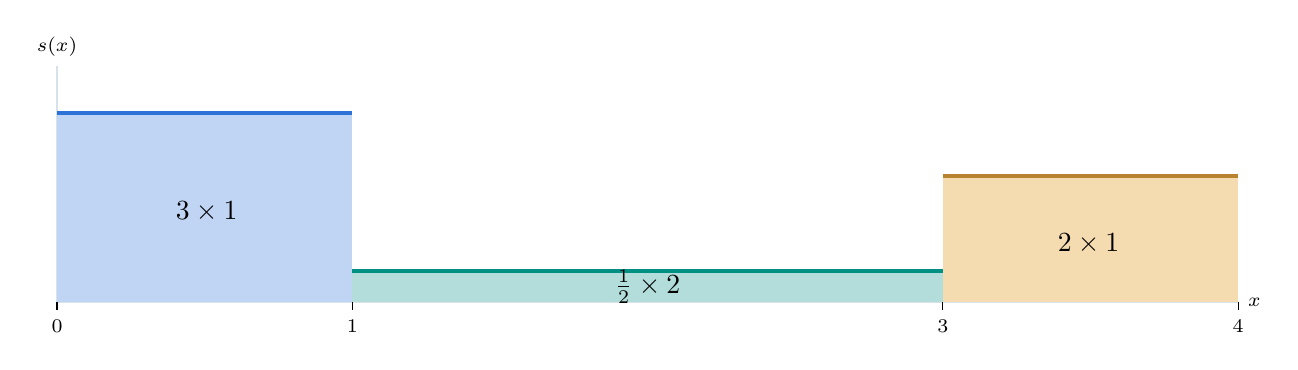
\begin{tikzpicture}[x=1cm,y=1cm]
\draw[axis] (0,0)--(15,0) node[right,font=\scriptsize] {$x$};\draw[axis] (0,0)--(0,3) node[above,font=\scriptsize] {$s(x)$};
\fill[blue!30] (0,0) rectangle (3.75,2.4);\fill[teal!30] (3.75,0) rectangle (11.25,.4);\fill[gold!40] (11.25,0) rectangle (15,1.6);
\draw[blue,line width=1.4pt] (0,2.4)--(3.75,2.4);\draw[teal,line width=1.4pt] (3.75,.4)--(11.25,.4);\draw[gold!80!black,line width=1.4pt] (11.25,1.6)--(15,1.6);
\foreach \x/\lab in {0/0,3.75/1,11.25/3,15/4}{\draw (\x,0)--(\x,-.1) node[below,font=\scriptsize]{\lab};}
\node at (1.9,1.15) {$3\times1$};\node at (7.5,.2) {$\tfrac12\times2$};\node at (13.1,.75) {$2\times1$};
\end{tikzpicture}
\end{center}
\newpage

\renewcommand{\footertext}{WORKED EXAMPLES / IMPROPER BEHAVIOUR / LAYER CAKE}
\pagehead{07}{SINGULARITIES AND TAILS}{What happens near infinity?}
\lead{Lebesgue theory handles unbounded functions naturally: truncate, integrate the bounded pieces, and pass upward by monotone convergence.}
\begin{minipage}[t]{.48\textwidth}
\begin{mathbox}\eyebrow{Example 3: a power singularity}\par
For $f(x)=x^{-p}$ on $(0,1)$, $p>0$, define $f_n=\min(f,n)$. Then $f_n\uparrow f$, so
\[\int_0^1x^{-p}\dd x=\lim_{\varepsilon\downarrow0}\int_\varepsilon^1x^{-p}\dd x.\]
If $p\ne1$, this equals
\[\lim_{\varepsilon\downarrow0}\frac{1-\varepsilon^{1-p}}{1-p}.\]
Hence
\[\boxed{\int_0^1x^{-p}\dd x<\infty\iff p<1}\]
\[\text{and, when }p<1,\qquad \int_0^1x^{-p}\dd x=\frac1{1-p}.\]
For $p=1$, the logarithm diverges.\end{mathbox}
\end{minipage}\hfill
\begin{minipage}[t]{.48\textwidth}
\begin{tealbox}\eyebrow{Example 4: layer cake}\par
Let $f(x)=e^{-x}$ on $[0,\infty)$. For $0<t<1$,
\[\{x:e^{-x}>t\}=[0,-\log t),\]
so its measure is $-\log t$. For $t\ge1$ it is empty. Thus
\begin{align*}
\int_0^\infty e^{-x}\dd x
&=\int_0^1(-\log t)\dd t\\
&=\boxed1.
\end{align*}
The same area is read from the widths of horizontal superlevel sets.\end{tealbox}
\end{minipage}
\vspace{8pt}
\begin{goldbox}\textbf{Tail test.} On $(1,\infty)$, $\int_1^\infty x^{-p}\dd x<\infty$ exactly when $p>1$. Near zero the threshold is $p<1$; at infinity it reverses. Always identify where the possible divergence lives.\end{goldbox}
\newpage

\renewcommand{\footertext}{MONOTONE CONVERGENCE / FATOU / DOMINATED CONVERGENCE}
\pagehead{08}{THE THREE LIMIT THEOREMS}{When may a limit pass through the integral?}
\lead{Pointwise convergence alone is too weak. These theorems provide three progressively different forms of control.}
\begin{center}
\renewcommand{\arraystretch}{1.35}
\begin{tabular}{>{\bfseries}p{31mm}p{52mm}p{66mm}}
\toprule
Theorem & Hypotheses & Conclusion \\
\midrule
Monotone convergence & $0\le f_n\uparrow f$ a.e. & $\displaystyle\int f_n\to\int f$; infinity is allowed.\\
Fatou's lemma & $f_n\ge0$ measurable & $\displaystyle\int\liminf f_n\le\liminf\int f_n$.\\
Dominated convergence & $f_n\to f$ a.e. and $|f_n|\le g$ with $g\in L^1$ & $f\in L^1$, $\displaystyle\int f_n\to\int f$, and $\|f_n-f\|_1\to0$.\\
\bottomrule
\end{tabular}
\end{center}
\begin{center}
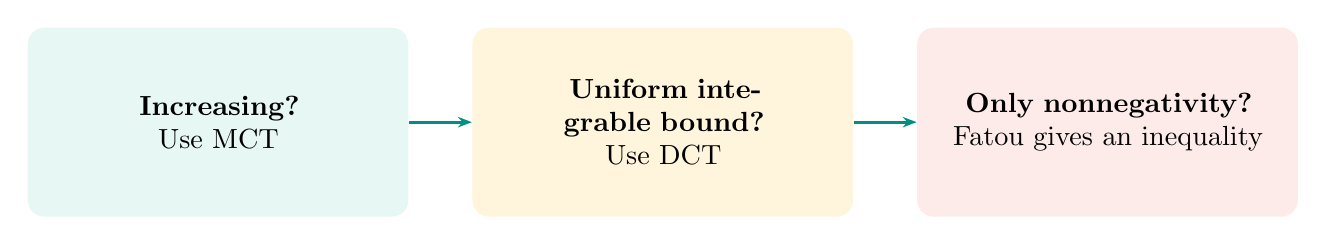
\begin{tikzpicture}[node distance=8mm]
\node[rounded corners=6pt,fill=paleteal,text width=46mm,minimum height=24mm,align=center] (m) {\textbf{Increasing?}\\Use MCT};
\node[rounded corners=6pt,fill=palegold,text width=46mm,minimum height=24mm,align=center,right=of m] (d) {\textbf{Uniform integrable bound?}\\Use DCT};
\node[rounded corners=6pt,fill=palecoral,text width=46mm,minimum height=24mm,align=center,right=of d] (f) {\textbf{Only nonnegativity?}\\Fatou gives an inequality};
\draw[flow] (m)--(d);\draw[flow] (d)--(f);
\end{tikzpicture}
\end{center}
\begin{coralbox}\eyebrow{Why pointwise convergence fails}\par
On $(0,1)$ let $f_n=n\1_{(0,1/n)}$. Then $f_n(x)\to0$ for every $x>0$, but $\int_0^1f_n\dd x=n(1/n)=1$. The mass grows taller while concentrating near zero. No single integrable function dominates the entire sequence.\end{coralbox}
\begin{quietbox}\textbf{Memory cue.} MCT controls direction; DCT controls size; Fatou gives the one-sided statement that survives with minimal control.\end{quietbox}
\newpage

\renewcommand{\footertext}{WORKED LIMITS / DOMINATION / SERIES}
\pagehead{09}{CALCULATING WITH CONVERGENCE}{Two complete limit exchanges}
\lead{The essential move is not evaluating the integral; it is naming the theorem and verifying every hypothesis.}
\begin{minipage}[t]{.48\textwidth}
\begin{tealbox}\eyebrow{Example 5: dominated convergence}\par
Compute $\lim_{n\to\infty}\int_0^1\frac{x^n}{1+x}\dd x$.
For $0\le x<1$, $x^n/(1+x)\to0$; the endpoint $x=1$ is a null exception. Also
\[0\le\frac{x^n}{1+x}\le1,\]
and $g(x)=1$ lies in $L^1[0,1]$. DCT gives
\[\boxed{\lim_{n\to\infty}\int_0^1\frac{x^n}{1+x}\dd x=0}.\]
No antiderivative is needed.\end{tealbox}
\end{minipage}\hfill
\begin{minipage}[t]{.48\textwidth}
\begin{goldbox}\eyebrow{Example 6: integrate a series}\par
For $0\le x<1$, $\sum_{k=0}^n x^k\uparrow(1-x)^{-1}$. On $[0,a]$ with $a<1$, MCT yields
\begin{align*}
\int_0^a\frac1{1-x}\dd x
&=\sum_{k=0}^\infty\int_0^a x^k\dd x\\
&=\sum_{k=0}^\infty\frac{a^{k+1}}{k+1}\\
&=\boxed{-\log(1-a)}.
\end{align*}
Nonnegative partial sums make MCT automatic.\end{goldbox}
\end{minipage}
\vspace{9pt}
\begin{mathbox}\eyebrow{A reusable dominated-convergence proof}\par
Write four sentences: (1) $f_n\to f$ pointwise a.e.; (2) every $f_n$ is measurable; (3) $|f_n|\le g$ a.e.; (4) $g\in L^1$. Therefore DCT gives $\int f_n\to\int f$. If any sentence is missing, the interchange is not yet justified.\end{mathbox}
\begin{coralbox}\textbf{Do not dominate by a constant on an infinite-measure space.} The function $1$ is integrable on $[0,1]$, but not on $\R$. Domination is global and measure-dependent.\end{coralbox}
\newpage

\renewcommand{\footertext}{FUBINI / TONELLI / PRODUCT MEASURE}
\pagehead{10}{ITERATED INTEGRALS}{When may the order be changed?}
\lead{Product measure turns area into repeated one-dimensional measurement. Tonelli handles nonnegative functions; Fubini handles absolutely integrable signed functions.}
\begin{mathbox}
\textbf{Tonelli:} if $f\ge0$ is measurable, then
\[\int_{X\times Y}f\dd(\mu\times\nu)=\int_X\!\left(\int_Yf(x,y)\dd\nu(y)\right)\dd\mu(x),\]
with values possibly infinite. \textbf{Fubini:} if $\int_{X\times Y}|f|<\infty$, both iterated integrals exist a.e., are integrable, and equal the double integral.
\end{mathbox}
\begin{tealbox}\eyebrow{Example 7: a triangular region}\par
Let $T=\{(x,y):0<x<1,\ 0<y<x\}$. Since $\1_T\ge0$, Tonelli allows either order:
\begin{align*}
m_2(T)&=\int_0^1\int_0^x1\dd y\dd x=\int_0^1x\dd x=\tfrac12,\\
&=\int_0^1\int_y^11\dd x\dd y=\int_0^1(1-y)\dd y=\boxed{\tfrac12}.
\end{align*}
\end{tealbox}
\begin{center}
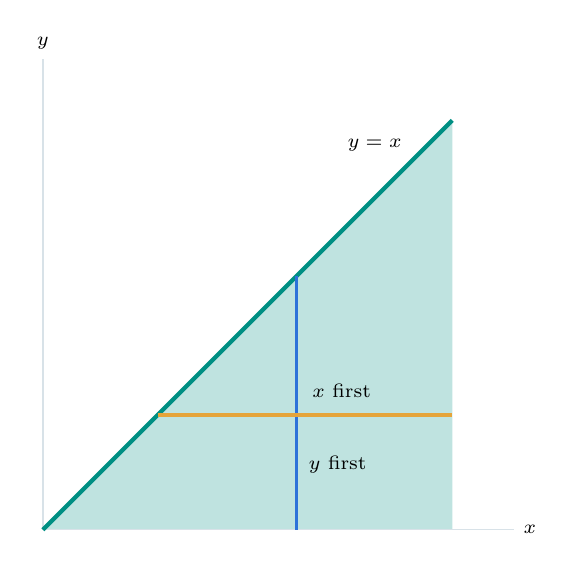
\begin{tikzpicture}[x=5.2cm,y=5.2cm]
\fill[teal!25] (0,0)--(1,0)--(1,1)--cycle;\draw[axis] (0,0)--(1.15,0) node[right,font=\scriptsize]{$x$};\draw[axis] (0,0)--(0,1.15) node[above,font=\scriptsize]{$y$};\draw[tealcurve] (0,0)--(1,1);\draw[blue,line width=1.2pt] (.62,0)--(.62,.62);\draw[gold,line width=1.2pt] (.28,.28)--(1,.28);\node[font=\scriptsize] at (.72,.16){$y$ first};\node[font=\scriptsize] at (.73,.34){$x$ first};\node[font=\scriptsize,above left] at (.9,.9){$y=x$};
\end{tikzpicture}
\end{center}
\begin{coralbox}\textbf{Warning.} Conditional cancellation can make two iterated integrals disagree or one fail to exist. For signed $f$, check $\int|f|<\infty$ before exchanging order.\end{coralbox}
\newpage

\renewcommand{\footertext}{$L^1$ / ABSOLUTE CONTINUITY / A CALCULATION CHECKLIST}
\pagehead{11}{THE FUNCTION SPACE VIEW}{Integrable functions form a complete space}
\lead{Lebesgue integration is not only a number-producing device. It creates the normed space $L^1$, where convergence in mean becomes a robust language for approximation.}
\begin{mathbox}\centering
$L^1(X,\mu)=\{f:\text{$f$ measurable and }\|f\|_1=\int_X|f|\dd\mu<\infty\}/\text{a.e. equality}.$
\end{mathbox}
\begin{minipage}[t]{.48\textwidth}
\begin{tealbox}\textbf{Core properties}\par
\begin{itemize}
\item $\|f\|_1\ge0$, with equality exactly when $f=0$ a.e.
\item $\|af\|_1=|a|\|f\|_1$.
\item $\|f+g\|_1\le\|f\|_1+\|g\|_1$.
\item $|\int f|\le\int|f|=\|f\|_1$.
\item $L^1$ is complete: every Cauchy sequence has an $L^1$ limit.
\end{itemize}\end{tealbox}
\end{minipage}\hfill
\begin{minipage}[t]{.48\textwidth}
\begin{goldbox}\textbf{Absolute continuity of the integral}\par
If $f\in L^1$, then for every $\varepsilon>0$ there is $\delta>0$ such that
\[\mu(A)<\delta\implies\int_A|f|\dd\mu<\varepsilon.\]
An integrable function cannot hide a fixed amount of mass in sets whose measure tends to zero. This explains why the spike sequence on page 9 has no $L^1$ dominator.\end{goldbox}
\end{minipage}
\vspace{7pt}
\begin{quietbox}\eyebrow{Final checklist}\par
\begin{enumerate}
\item Name the measure space and the set of integration.
\item Establish measurability; split into positive and negative parts if needed.
\item Test $\int|f|$ when a finite signed answer or Fubini is required.
\item Calculate by simple sums, classical calculus, layer cake, or iteration.
\item For limits, state pointwise/a.e. convergence and verify MCT, Fatou, or DCT hypotheses explicitly.
\item Sanity-check sign, scale, null-set invariance, and possible infinite values.
\end{enumerate}\end{quietbox}
\newpage

\renewcommand{\footertext}{SUMMARY / EXERCISES / REFERENCES}
\pagehead{12}{THE WHOLE THEORY AT A GLANCE}{A compact map and practice set}
\begin{center}
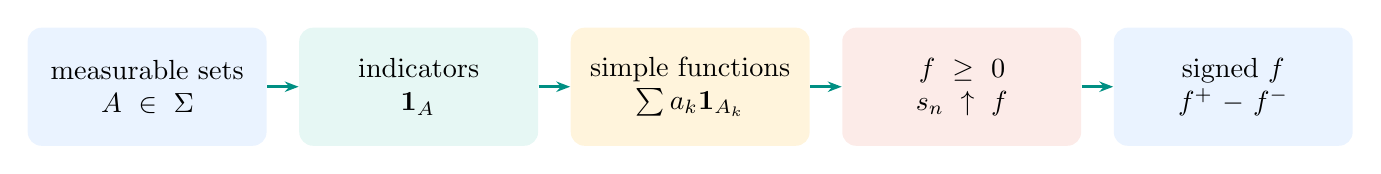
\begin{tikzpicture}[node distance=4mm]
\node[rounded corners=5pt,fill=paleblue,text width=28mm,minimum height=15mm,align=center] (sets) {measurable sets\\$A\in\Sigma$};
\node[rounded corners=5pt,fill=paleteal,text width=28mm,minimum height=15mm,align=center,right=of sets] (ind) {indicators\\$\1_A$};
\node[rounded corners=5pt,fill=palegold,text width=28mm,minimum height=15mm,align=center,right=of ind] (simp) {simple functions\\$\sum a_k\1_{A_k}$};
\node[rounded corners=5pt,fill=palecoral,text width=28mm,minimum height=15mm,align=center,right=of simp] (nonneg) {$f\ge0$\\$s_n\uparrow f$};
\node[rounded corners=5pt,fill=paleblue,text width=28mm,minimum height=15mm,align=center,right=of nonneg] (signed) {signed $f$\\$f^+-f^-$};
\foreach \a/\b in {sets/ind,ind/simp,simp/nonneg,nonneg/signed}{\draw[flow](\a)--(\b);}
\end{tikzpicture}
\end{center}
\begin{tealbox}\textbf{One sentence.} Measure assigns size to sets; measurable functions pull value thresholds back to measurable sets; simple functions weight those sets; arbitrary nonnegative functions are limits from below; signed integrable functions are differences with finite total absolute mass.\end{tealbox}
\begin{multicols}{2}
\textbf{Practice}
\begin{enumerate}
\item Compute $\int_{[0,2]}(2\1_{[0,1]}+5\1_{(1,2]})\dd x$.
\item Find $\int_0^1\1_{\R\setminus\mathbb Q}\dd x$.
\item For which $p$ is $x^{-p}$ integrable on $(0,1)$? On $(1,\infty)$?
\item Justify $\lim_n\int_0^1x^n\sin x\dd x=0$.
\item Use Tonelli to compute the area under $y=1-x^2$ on $[0,1]$.
\end{enumerate}
\columnbreak
\textbf{Answers}
\begin{enumerate}
\item $2(1)+5(1)=7$.
\item $1$, because the irrationals have full measure.
\item $p<1$ near zero; $p>1$ at infinity.
\item Pointwise a.e. convergence to $0$ and domination by $1\in L^1[0,1]$; apply DCT.
\item $\int_0^1(1-x^2)\dd x=2/3$.
\end{enumerate}
\end{multicols}
\begin{quietbox}\eyebrow{References for the next step}\par
G. Folland, \emph{Real Analysis}, 2nd ed.; H. Royden and P. Fitzpatrick, \emph{Real Analysis}, 4th ed.; T. Tao, \emph{An Introduction to Measure Theory}; W. Rudin, \emph{Real and Complex Analysis}, 3rd ed.\end{quietbox}
\vfill
{\fontsize{8}{10}\selectfont\color{muted}This guide emphasizes the conceptual and computational core. Standard results are stated for complete measure spaces where convenient; consult the references for construction of Lebesgue measure, completion, and full proofs.}
\end{document}
